\documentclass[english]{tex/bluebook}

\usepackage{blindtext}

\title{The Blue Book}
\author{John Doe}
\date{2020}


\begin{document}
	\maketitle	
	\frontmatter
	\tableofcontents

	\mainmatter
	\part{First things first}
	\chapter{Basic Layout and Usage}
	The basic layout is intended for using it in non-fiction but not necessarily for university purposes. 
	Both, footnotes\footnote{Like this one} and endnotes\endnote{Endnotes are often used to keep the flow of a text while providing additional information like sources or remarks. 
	In this \enquote{template} they are sorted by chapter.} are supported but the usage of endnotes over footnotes is encouraged. To improve navigation, the endnote section features the backref \index{Backref}feature and it is therefore possible to jump back to the note in text when using a PDF version of the book. 	\index{Footnote} \index{Endnote}
	By now only three variables should be set to receive a fully featured PDF book (well and of course one needs to insert the actual content \dots). 
	Title, author and date as it is usually done when using the standard \LaTeX{} classes or \KOMAScript{}. The cover, back cover and title page utilize those information automatically. 
	
	Bluebook is not particularly a template but more of a personal exercise in \LaTeX. The source of this document should give enough inside on how to use it if you're interested. The remainder of this example is filled with blindtext to illustrate the typography and general appearance.	
	
	\begin{figure}
		\centering
		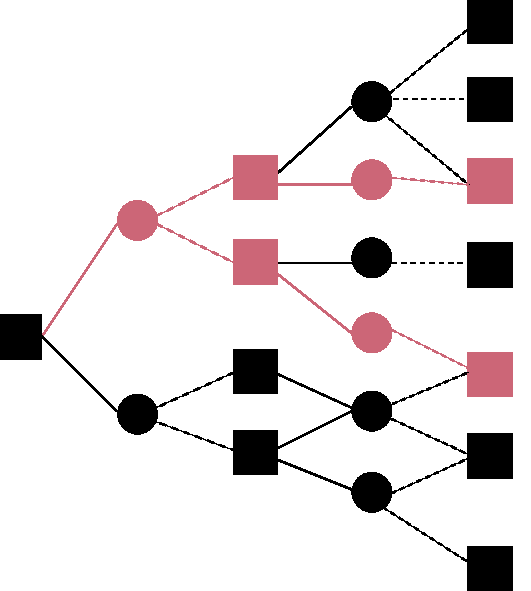
\includegraphics[width=0.70\linewidth]{la_rollout}
		\caption{An example image. This is an illustration of a rollout policy in Approximate Dynamic Programming. It doesn't really matter and is only here to highlight the referencing of images.}
		\label{fig:la_rollout}
	\end{figure}	

	\chapter{Example Chapter}
	\blindtext[25]
	
	\part{Some Filler}
	\chapter{Another Example Chapter}
	\blindtext[28]
	
	\cleardoublepage
	\printendnotes	
	\printindex
	\cleardoubleemptypage
	\closeBook{This is the dust cover blurb. It should shortly outline the contents of the book to interest the reader. For this \enquote{template} the \emph{closeBook} command is used to generate the page you are reading right now.}
\end{document}
